\documentclass[../../main.tex]{subfiles}

\subsection{Introducción}
\vspace{2mm}
\noindent
Al realizar una aplicación para probar la arquitectura propuesta partimos de la premisa de que la misma fuese híbrida, dado que resultaba interesante
tan solo desarrollar una vez y ser capaz de desplegar en varias plataformas. Para ello vamos a intentar explicar las cuatro alternativas más utilizadas
en este tipo de desarrollo. A continuación veremos cuáles son los puntos fuertes y débiles de cada una de estas alternativas.

\subsubsection{Apache Cordova}
\noindent
\textit{Apache Cordova} es una aproximación opensource al desarrollo multiplatafor\-ma,
su mayor ventaja es la simplicidad con respecto a las otras alternativas. Permite crear
aplicaciones de todo tipo de corte, no solo móviles, sino también de escritorio o
incluso web. Para ello utiliza Web APIs, y es capaz de envolver aplicaciones web en
una aplicación nativa de la plataforma en cuestión y utiliza por sí sola la API
correspondiente de la plataforma en cuestión cuando se la llama.

Las aplicaciones \textit{Cordova} son simplemente una colección de páginas HTML que
son renderizadas en el teléfono móvil como WebViews. Para desarrollar las aplicaciones
solo te hace falta HTML5, CSS y JavaScript. Entre las expuestas es la única que
sigue completamente la filosofía “write once, run anywhere”.\\

\textbf{Ventajas}

\begin{itemize}

\item Pequeña y simple API nativa que permite ser usada en diferentes entornos de desarrollo.
\item Alta reusabilidad con HTML, CSS y JavaScript.
\item Cualquier cosa escrita como una página web puede ser fácilmente envuelta como una aplicación nativa de la plataforma para la que estamos desarrollando.
\item Soporte para todas las plataformas y sistemas operativos que incluyen Android, iOS, Windows Phone, Blackberry, Firefox OS y Ubuntu.
\item La mayoría de desarrolladores están acostumbrados a codificar en HTML/CSS/JavaScript por lo que tienen muy fácil el hecho de empezar a trabajar en \textit{Cordova}.
    
\end{itemize}

\textbf{Desventajas}

\begin{itemize}

\item Peor rendimiento que aplicaciones de código nativo ya que al fin y al cabo son aplicaciones web que se lanzan con el motor del navegador del dispositivo.
\item Muchas librerías muy fragmentadas con frameworks de nivel básico.
\item Interfaces de Usuario que pueden distar mucho de la apariencia nativa de la plataforma, aunque esto depende mucho del desarrollador en sí.
    
\end{itemize}

\subsubsection{Titanium Appcelerator}
\noindent
Titanium es una plataforma de desarrollo basada en JavaScript. Titanium utiliza
JavaScript para escribir código de aplicaciones que después utilizan la API y la UI
de una y solo una de las plataformas a las que va destinada. Es decir, al
contrario que \textit{Cordova}, esta plataforma de desarrollo no está orientada a la
filosofía “write once and run anywhere”, aunque da la posibilidad de reutilizar las
partes comunes entre las plataformas que intentamos desarrollar.

Tiene la desventaja que al contrario que \textit{Cordova} y Xamarin tendremos que
aprender parte de la API de cada una de las plataformas que vamos a desarrollar
y no solo eso, sino que tendremos que aprender la capa que envuelve a esas APIs
en JavaScript que es como las terminaremos utilizando.\\

\textbf{Ventajas}

\begin{itemize}
\item Mejor rendimiento, ya que se hace un uso de las APIs de cada plataforma de manera nativa. También tenemos la ventaja que da acceso específico a características propias de cada plataforma.
\item La apariencia de las aplicaciones realizadas con Titanium es puramente nativo en cada plataforma, y no tendremos que dedicar mucho tiempo a que esto sea así.
\item Con JavaScript se asegura un desarrollo fácil y rápido.
    
\end{itemize}

\textbf{Desventajas}

\begin{itemize}

\item No tiene soporte para librerías de terceros.
\item Dificultad a la hora de desarrollar aplicaciones complejas.
\item Ya que no utiliza HTML5 o CSS, la animaciones y los elementos del DOM muchas veces actúan con un poco de retardo, en general responden de manera más lenta.
    
\end{itemize}

\subsubsection{Microsoft Xamarin}
\noindent
Xamarin, conocido originalmente como MonoTouch es otro framework multiplataforma que
se ha hecho un hueco en el mercado con su propio IDE. Funciona con C\# todo
dentro del “.NET Framework” y te permite realizar aplicaciones nativas utilizando
las APIs y UIs de cada plataforma.

Xamarin viene con la librería Xamarin.Forms que nos permite escribir UIs para
una plataforma de manera nativa y después compartirlas con el resto de
plataformas que queremos desarrollar. Xamarin soporta iOS, Android y
plataformas Windows.\\

\textbf{Ventajas}

\begin{itemize}
\item Xamarin incluye TestCloud que nos permite probar aplicaciones de manera automática.
\item Proporciona código $100\%$ reutilizable en el desarrollo de UIs gracias a
Xamarin.Forms, lo cual nos ahorrará mucho tiempo y esfuerzo.
\item Soporta patrones como MVC y MVVM.
Xamarin.Android soporta Goo\-gle Glass, Android Wear y Firephone.
\item La curva de aprendizajes es muy relativa. Si conoces C\# resulta bastante
fácil comenzar a desarrollar con Xamarin.
\end{itemize}
\newpage
\textbf{Desventajas}

\begin{itemize}
\item No permite acceso directo a controles específicos de elementos de la UI de
Android.
\item Utilizar Xamarin provoca ciertos retrasos en los tiempos de carga cuando
la app está en ejecución.
\item No permite compartir ni desarrollar código fuera del entorno de desarrollo
Xamarin.
\end{itemize}

\subsubsection{Ionic}
\noindent
\textit{Ionic} \cite{ionic_2017} es un framework desarrollado sobre \textit{Apache Cordova}, por lo que comparten sus puntos fuertes y débiles.
No obstante el desarrollo se basa en dos frameworks que van de la mano. Por un lado \textit{Angular} \cite{ngbook_2016}, framework desarrollado
por Google, el cual está completamente basado en componentes auto-contenidos, básicamente todo lo que desarrollamos con él (páginas, servicios, items, etc) terminan convirtiéndose en componentes, a veces
individuales y otras como parte de otros componentes. Por otro lado, el propio \textit{Ionic} es otro framework que se construye sobre el propio \textit{Angular} donde todos sus componentes
vienen a ser componentes \textit{Angular}, pero que en el caso de componentes gráficos estos se adaptan a la plataforma en la cual son desplegados.
Una ventaja es que podemos mezclar indistintamente componentes de ambos lenguajes (tanto \textit{Angular} como \textit{Ionic}). En ambos trabajamos en TypeScript, un lenguaje de alto nivel extensión de Javascript.

La idea es que desarrollamos una aplicación web basándonos en componentes \textit{Angular} y \textit{Ionic}, en la que el cliente de \textit{Ionic} a la hora de construir
el proyecto va a realizar optimizaciones basándose en la plataforma para la que están siendo construidos. Con lo cual es una solución que se acerca mucho más al
comportamiento de los componentes nativos incluso donde \textit{Cordova} tiene problemas, que es normalmente en los componentes gráficos. Respecto al uso de componentes de tipo dispositivo, dentro
de la plataforma donde estamos desarrollando, véase cosas como cámara, gps, acelerómetros, etc. el comportamiento es idéntico al de \textit{Cordova}, no hay ningún impacto significativo con respecto al uso nativo de los mismos.\\
\newpage
\textbf{Ventajas}

\begin{itemize}
\item Aplicaciones mucho más rápidas a la hora de desarrollar.
\item Las aplicaciones cuentan con un aspecto que corresponde a las plataformas en las cuales van a ser desplegadas.
\item Gran cantidad de plugins desarrollados para hacer uso de los sensores internos de los dispositivos.
\item El catálogo de librerías compatibles con \textit{Ionic} es muy extenso. 
\item Cliente de \textit{Ionic} muy robusto, lo que permite generar un código inicial de los componentes bastante completo.
\end{itemize}

\textbf{Desventajas}

\begin{itemize}
\item Peor rendimiento que aplicaciones de código nativo.
\item Necesidad de seguir la nomenclatura y la estructura de proyecto que exige \textit{Ionic}.
\item No recomendable para el desarrollo de videojuegos o de compoentes 3D ya que se ralentiza enormemente el rendimiento.
\end{itemize}
\noindent
En la tabla de la Figura \ref{tab:comparativa_hibridas} se observan las principales diferencias entre las distintas tecnologías de desarrollo híbrido.
\begin{figure}[H]
    \centering
    \caption{Tabla comparativa de tecnologías híbridas.}
    \label{tab:comparativa_hibridas}
    \resizebox{\textwidth}{!}{%
    \begin{tabular}{@{}r|lll@{}}
    \toprule
    \multicolumn{1}{l}{}               & \textbf{ Apache Cordova / Ionic}                                          & \textbf{Appcelerator}                & \textbf{Xamarin}                 \\ \midrule \toprule
    \textbf{Plataformas soportadas}    &$\begin{array}{l}
        \textrm{iOS, Android, Windows Phone,} \\ 
        \textrm{Blackberry, OSX, Windows,}\\
        \textrm{Linux,Ubuntu Phone...}\\
        \end{array}$                                                                                               & Blackberry                           & Android, iOS, Windows            \\ \midrule
    \textbf{Lenguaje de programación}  &$\begin{array}{l}
        \textrm{HTML5, CSS,} \\ 
        \textrm{JavaScript / Angular}\\
        \end{array}$                                                                                               & JavaScript                           & C\#                              \\ \midrule
    \textbf{UI}                        &$\begin{array}{l}
        \textrm{Web UI /} \\ 
        \textrm{Parcialmente nativa}\\
        \end{array}$                                                                                               & Nativa                               & Nativa                           \\ \midrule
    \textbf{Acceso a API del sistema}  &$\begin{array}{l}
        \textrm{Limitada a componentes} \\ 
        \textrm{desarrollados para la}\\
        \textrm{plataforma en concreto}\\
        \end{array}$                                                                                               & Completa                             & Completa                         \\ \midrule
    \textbf{Soporte de estandares web} &$\begin{array}{l}
        \textrm{SI} \\ 
        \end{array}$                                                                        & NO                                   & NO                               \\ \midrule
    \textbf{Soporte del DOM}           &$\begin{array}{l}
        \textrm{SI} \\ 
        \end{array}$                                                                        & NO                                   & SI                               \\ \midrule
    \textbf{Desempeño nativo}          &$\begin{array}{l}
        \textrm{NO} \\ 
        \end{array}$                                                                        & SI                                   & SI                               \\ \midrule
    \textbf{Usado por}                 &$\begin{array}{l}
        \textrm{IBM, Sony, Mozilla, Intel...} \\ 
        \end{array}$                                             & Cisco, VMWare, MitsubishiElectric... & GitHub, Microsoft, FourSquare... \\ \midrule
    \toprule
    \end{tabular}%
    }
\end{figure}
\noindent
Una vez vista las principales diferencias entre las distintas tecnologías para el desarrollo de aplicaciones híbridas decidimos utilizar la alternativa de \textit{Ionic} ya que nos permite sin excesivos esfuerzos
desarrollar una aplicación básica para probar nuestro back-end, que a su vez, sin mucho esfuerzo, va a tener un aspecto nativo a la plataforma donde se despliegue.\\

\subsection{¿Que es Whaya?}
\vspace{2mm}
\noindent
Whaya es una aplicación desarrollada con el objetivo principal de probar la arquitectura de microservicios propuesta anteriormente. A pesar de ello, la aplicación presenta una cierta funcionalidad importante
como detallaremos más adelante. Para desarrollarla, como comentábamos anteriormente, hemos elegido \textit{Ionic} que es un framework de desarrollo híbrido de aplicaciones que hace uso de \textit{Angular} para generar aplicaciones móviles basadas en componentes.
De manera nativa \textit{Ionic} nos ofrece la posibilidad de utilizar todo tipo de funcionalidades de nuestro dispositivo móvil mediante la instalación de plugins, que no vienen a ser otra cosa
que nuevos componentes que nos permiten seguir montando el \textbf{rompecabezas} mediante el cual desarrollamos nuestra aplicación. Dado que no todo es el uso de los recursos hardware
de nuestro dispositivo también contamos por defecto con componentes gráficos, los cuales \textit{Ionic} se encarga a la hora de compilar nuestra aplicación hacer que esta luzca de la manera
que esperamos en dispositivo en el que la vamos a desplegar. La Figura \ref{fig:androidVsIosFe} muestra una comparativa entre la interfaz de la versión Android y la iOS, en ellas podemos
apreciar particularidades de cada una de las plataformas, como pueden ser dónde están situados los títulos de las cabeceras de las ventanas de la aplicación, iconos de las mismas, menús adaptados a plataformas, etc.

\begin{figure}[H]
    \centering{%
    \setlength{\fboxsep}{0pt}%
    \setlength{\fboxrule}{1pt}%
    \subfloat[Interfaz android]{\fbox{{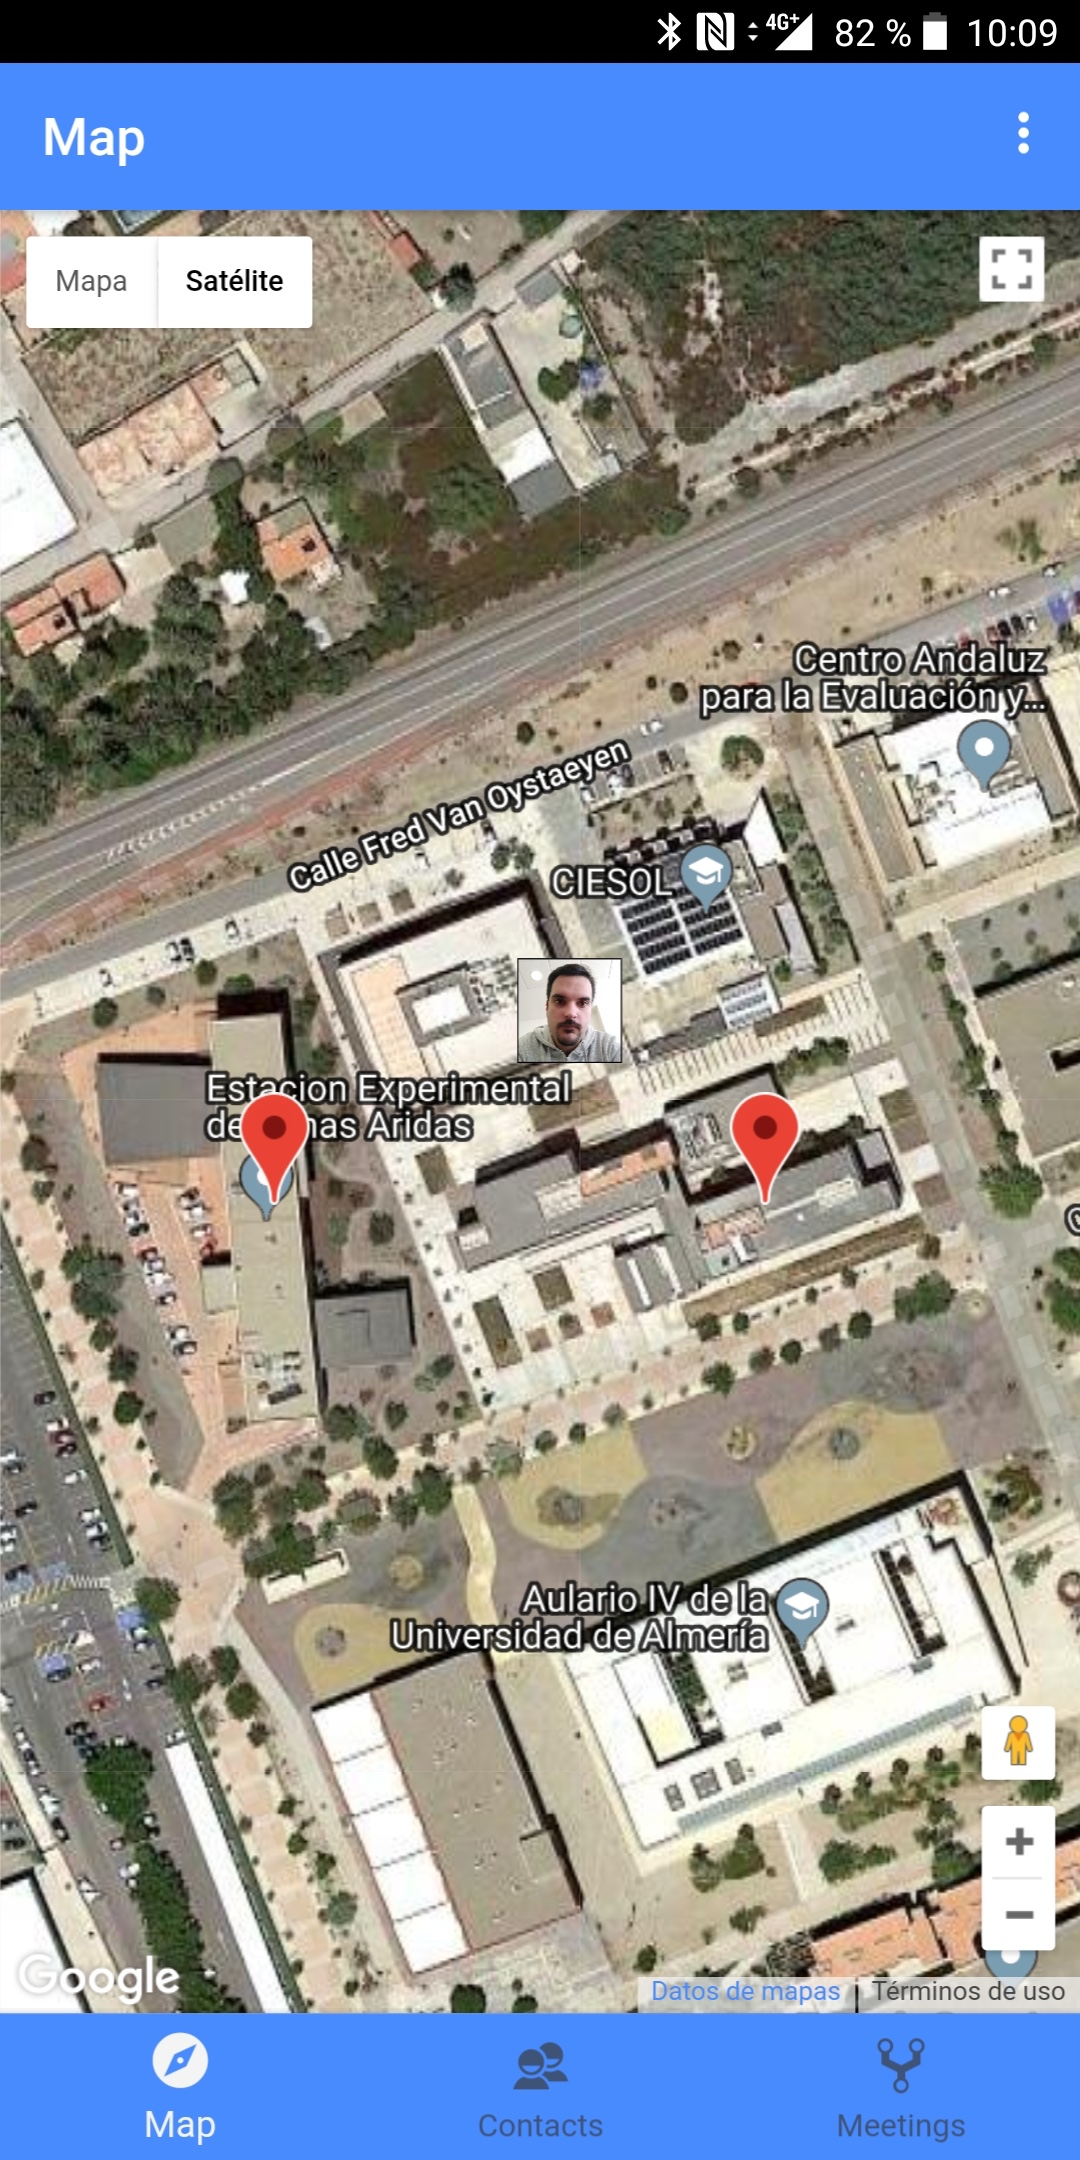
\includegraphics[width=0.4\textwidth]{androidlook} }}}%
    \qquad
    \subfloat[Interfaz ios]{\fbox{{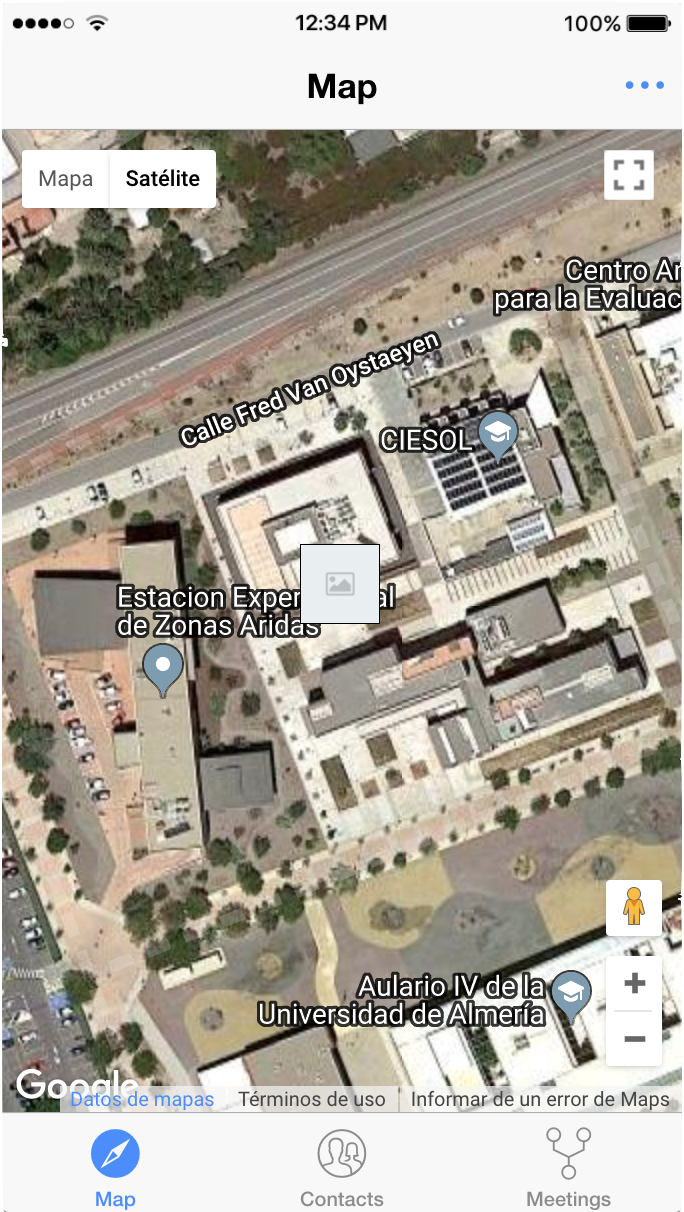
\includegraphics[width=0.4\textwidth]{ioslook} }}}%
    \qquad
    \caption{Android vs iOS.}%
    \label{fig:androidVsIosFe}%
    }%
\end{figure}
\noindent
La posibilidad de que, de manera automática se adapte la interfaz a la plataforma donde se ejecuta la aplicación al utilizar los componentes nativos de \textit{Ionic}, proporciona una descarga de trabajo sustancial de cara a
diseñar la interfaz de usuario, y aún así proporcionar a los usuarios que utilicen la aplicación una experiencia de uso familiar.

Después de comentar las particularidades de \textit{Ionic} vamos a pasar a nombrar los casos de uso que nuestra aplicación desarrolla, los cuales presentamos en la Figura \ref{fig:casoUsoWhaya}.

\begin{figure}[H]
    \centering
    {%
    \setlength{\fboxsep}{0pt}%
    \setlength{\fboxrule}{1pt}%
    \fbox{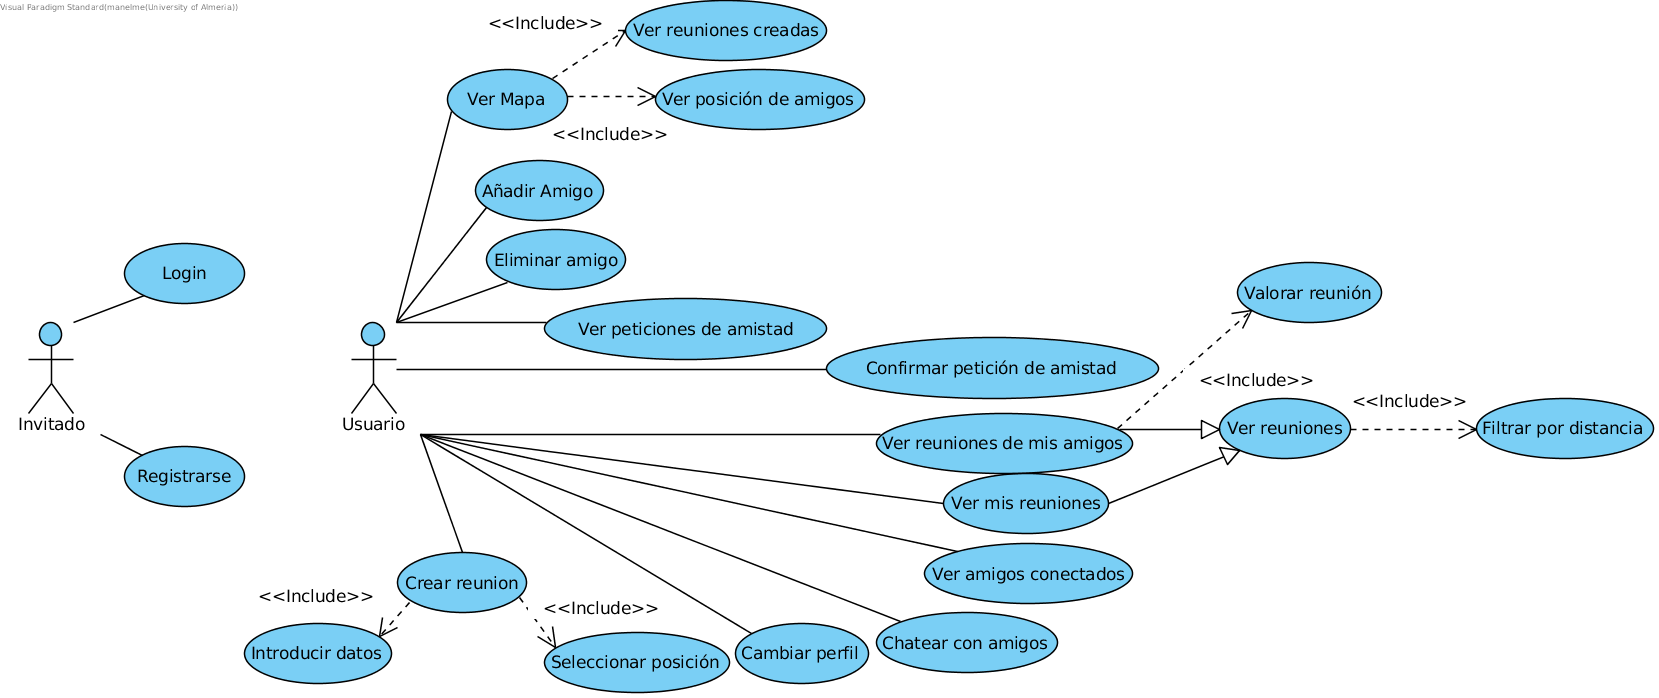
\includegraphics[width=\textwidth]{casoUsoWhaya}
    }%
    }%
    \caption{Diagrama de casos de uso Whaya.}
    \label{fig:casoUsoWhaya}
\end{figure}
\noindent
Consideramos el nombre de cada uno de los casos de uso lo suficientemente descriptivo como para no tener que entrar en profundidad en cada uno de ellos, ya que queda un poco fuera del alcance de este proyecto.\\

\subsection{Desarrollo de Whaya}
\vspace{2mm}
\noindent
Para entender mejor como se desarrolla una aplicación con \textit{Ionic} vamos a intentar explicar cómo hemos desarrollado alguna de las páginas de nuestra aplicación, así como consideraciones que hay que tener en cuenta
a la hora de realizar implementaciones con \textit{Ionic}.

En primer lugar tenemos que instalar \texttt{Node.js}, para a continuación instalar de manera global el intérprete de \textit{Ionic} junto con su base \textit{Cordova}. Esto ya se encarga de descargar todas las dependencias necesarias para hacer funcionar la aplicación en nuestro
sistema. Para ello, y dado a que nuestra máquina de desarrollo está basada en Ubuntu, lo único que tenemos que hacer es ejecutar las ordenes pertinentes de instalación.

\begin{lstlisting}
    curl -sL https://deb.nodesource.com/setup_9.x | sudo -E bash -
    sudo apt-get install -y nodejs
    npm install -g cordova Ionic
\end{lstlisting}

Una vez realizamos la instalación de los intérpretes necesarios, nos situamos en la carpeta donde queremos guardar nuestro proyecto y ejecutamos la orden de iniciación del proyecto. En la misma tenemos que
disparar también el arquetipo que deseamos utilizar de inicio. En nuestro caso iniciamos nuestra aplicación con el arquetipo tabs, y declaramos el nombre de nuestra aplicación.

\begin{lstlisting}
    Ionic start Whaya tabs
\end{lstlisting}
\noindent
Esto nos va a generar todo la estructura de carpetas junto con los archivos básicos necesarios en el proyecto. En la Figura \ref{fig:scaffoldingWhayaFe} apreciamos cuales son los archivos y carpetas mínimos necesarios, y sabiendo que en la raíz del proyecto hay que prestar especial atención a 4 cosas:

\begin{enumerate}[label=\alph*)]
    \item \textbf{config.xml}. En este archivo se guarda la configuración del proyecto, tanto de manera global, como configuraciones de plataformas en concreto. Configuraciones correspondientes al nombre y versión de la aplicación, así como mensajes de permisos de uso de un componente hardware de la aplicación.
    \item \textbf{package.json}. En este archivo tenemos las dependencias directas de nuestro proyecto
    \item \textbf{resources/}. En esta carpeta se guardan archivos de recursos generados por el cliente de \textit{Ionic}, del estilo de iconos de la aplicación o pantallas de carga de la misma.
    \item \textbf{src/}. Esta carpeta contiene los componentes en los cuales implementamos nuestra aplicación, páginas, servicios, etc.
\end{enumerate}

\begin{figure}[H]
    \centering
    {%
    \setlength{\fboxsep}{0pt}%
    \setlength{\fboxrule}{1pt}%
    \fbox{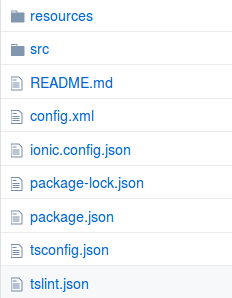
\includegraphics[width=0.3\textwidth]{scaffoldingWhayaFe}
    }%
    }%
    \caption{Scaffolding de Whaya.}
    \label{fig:scaffoldingWhayaFe}
\end{figure}
\noindent
El siguiente paso antes de iniciar el proceso de programación de nuestra aplicación será indicarle al proyecto \textit{Ionic} cuales son las plataformas
objetivo, en nuestro caso Android e iOS. Para ello utilizamos la siguiente orden.

\begin{lstlisting}
    Ionic cordova platform add android
\end{lstlisting}
\noindent
Esta orden, de manera automática, va a generar una serie de líneas correspondientes a la plataforma que hemos elegido dentro del archivo \texttt{config.xml} teniendo en cuenta,
plugins que hayamos añadido previamente al proyecto, configurándolos de manera adecuada a la plataforma. Una vez hemos realizado estos pasos previos entramos en faena con la aplicación propiamente dicha.

Como hemos dicho antes, toda aplicación \textit{Ionic} se basa en el desarrollo de componentes, estos son pequeños fragmentos de código que aportan una funcionalidad. En nuestra aplicación hemos hecho uso principalmente de 4 tipos, a saber:

\begin{enumerate}[label=\alph*)]
    \item \textbf{Pages} (Listing \ref{lst:MeetingsPage}). Componentes que engloban todo lo necesario con la interacción con el usuario, en el siguiente fragmento de código apreciamos cómo se declaran estos componentes y a la vez de qué archivos se componen.
    Como se puede observar, lo primero que vemos después de los \texttt{import} es la inclusión de una serie de decoradores, \texttt{@IonicPage} indica que estamos hablando de un componente página. Ademas, podemos apreciar que tiene dos archivos principales:
    la ``vista", que la podemos encontrar donde indica \texttt{templateUrl} y el ``controlador" que viene a ser la clase que se exporta, que de cara a archivos externos la utilizaremos con el nombre indicado en el campo \texttt{selector}.
    
    \begin{minipage}{\linewidth}
    \begin{lstlisting}[language=JavaScript,basicstyle=\ttfamily\scriptsize, caption={Ejemplo componente Page \texttt{MeetingsPage.ts}.},captionpos=b, label={lst:MeetingsPage}]
        import { Component, ViewChild, ElementRef } from '@angular/core';
        import { IonicPage, NavController, NavParams } from 'Ionic-angular';
        import { GeolocProvider } from '../../providers/geoloc/geoloc'; ...
        @IonicPage()
        @Component({
          selector: 'page-meetings',
          templateUrl: 'meetings.html',
        })
        export class MeetingsPage {
          @ViewChild('ranger') ranger: ElementRef;
          constructor(public navCtrl: NavController, public navParams: NavParams, private storage: Storage, private geolocProvider: GeolocProvider, private neoService: NeoServiceProvider) {}
          ...
        }
    \end{lstlisting}
    \end{minipage}

    \item \textbf{Providers} (Listing \ref{lst:NeoServiceProvider}). En el mundo \textit{Angular} se denominan servicios, y cumplen con la funcionalidad de comunicarse con servicios web o con servicios internos del móvil como pueden ser la cámara, GPS, etc. En este caso
    vemos que simplemente hemos de declararlo como un archivo \texttt{@Injectable}, lo cual indica que está preparado para ser usado por otros componentes, cómo pueden ser por ejemplo las \texttt{pages}.
    
    \begin{minipage}{\linewidth}
    \begin{lstlisting}[language=JavaScript,basicstyle=\ttfamily\scriptsize, caption={Ejemplo componente Provider \texttt{NeoServiceProvider.ts}.},captionpos=b,label={lst:NeoServiceProvider}]
        import { Injectable } from '@angular/core';
        import { Http, Headers } from '@angular/http';...
        
        @Injectable()
        export class NeoServiceProvider {
            private headers = new Headers();
        private userAuth: any;
        constructor(public http: Http, public storage: Storage) {}
        ...
        }
    \end{lstlisting}
    \end{minipage}

    \item \textbf{Pipes} (Listing \ref{lst:RelativeTime}). Este tipo de componentes son los que se encargan básicamente de transformar datos antes de mostrarlos al usuario. En el ejemplo vemos como se declaran con el decorador @Pipe y a la vez lo dotamos de un nombre relativo.
    
    \begin{minipage}{\linewidth}
    \begin{lstlisting}[language=JavaScript,basicstyle=\ttfamily\scriptsize, caption={Ejemplo componente Pipe \texttt{RelativeTime.ts}.},captionpos=b,label={lst:RelativeTime}]
        import { Pipe, PipeTransform } from '@angular/core';
        import * as moment from 'moment';
        @Pipe({
          name: 'relativeTime',
        })
        export class RelativeTime implements PipeTransform {
          /**
           * Takes a value and makes it lowercase.
           */
          transform(value: string, ...args) {
              return moment(value).fromNow();
          }
        }
    \end{lstlisting}
    \end{minipage}

    \item \textbf{Components} (Listing \ref{lst:EmojiPickerComponent}). En nuestro caso hemos utilizado otro tipo de componente que queda un poco fuera de \textit{Ionic}, y podríamos considerarlo más como un componente \textit{Angular}. Básicamente, es una manera de generar otra capa de separación o abstracción. En nuestro caso lo uso para separar aquellos componentes (visuales) que por sí solos no significan nada, y que dependen del uso que otros hagan de ellos. Por ejemplo, un \texttt{@Component} puede ser la relación que tiene \texttt{emojiPicker} con \texttt{ChatPage}.
    Como ejemplo de \texttt{@Component} tenemos el siguiente, que es un componente que nos permite elegir un emoji para el chat.
    
    \begin{minipage}{\linewidth}
    \begin{lstlisting}[language=JavaScript,basicstyle=\ttfamily\scriptsize, caption={Ejemplo componente Component \texttt{EmojiPickerComponent.ts}.},captionpos=b, label={lst:EmojiPickerComponent}]
        import { Component, forwardRef } from '@angular/core';
        import { EmojiProvider } from "../../providers/emoji";
        import { ControlValueAccessor, NG_VALUE_ACCESSOR } from "@angular/forms";

        export const EMOJI_PICKER_VALUE_ACCESSOR: any = {
            provide: NG_VALUE_ACCESSOR,
            useExisting: forwardRef(() => EmojiPickerComponent),
            multi: true
        };

        @Component({
            selector: 'emoji-picker',
            providers: [EMOJI_PICKER_VALUE_ACCESSOR],
            templateUrl: './emoji-picker.html'
        })
        export class EmojiPickerComponent implements ControlValueAccessor {

            emojiArr = [];

            _content: string;
            _onChanged: Function;
            _onTouched: Function;
        constructor(emojiProvider: EmojiProvider) {
        this.emojiArr = emojiProvider.getEmojis();
        }
        ...
        }
    \end{lstlisting} 
    \end{minipage}
\end{enumerate}
\noindent
Como vemos, el lenguaje utilizado para definir los distintos componentes es TypeScript, extensión de Javascript que proporciona
ciertas funcionalidades adicionales de ES6 (EcmaScript 6), como es el tipado de objetos web para detectar errores en tiempo de compilación, el uso de clases, etc.
También hemos hecho uso, aunque solo donde es adecuado, de variables de tipo \texttt{Promises}, las cuales nos permiten dotar de cierta sincronía a algunas peticiones web,
y variables \texttt{Observables} que dotan a la aplicación de la posibilidad de actuar frente a cambios de valor de una variable.

También cabe destacar que tenemos dos maneras distintas de cargar nuestros componentes \textit{Ionic} en la aplicación:

\begin{itemize}
    \item Por un lado, contamos con la forma tradicional, que es cargar el componenente al cargar la aplicación, para ello tenemos que declararlo como un entryComponent en el archivo \texttt{app.module.ts}.
    Este archivo actúa como director de la aplicación y en él declararemos todos los componentes que nuestra aplicación hará uso de manera global. En el siguiente ejemplo (Listing \ref{lst:appModule}) podemos
    ver como el componente HomePage es declarado como un entryComponent en nuestra aplicación, esto quiere decir que se cargará cuando la misma se ejecute.

    \begin{lstlisting}[language=JavaScript,basicstyle=\ttfamily\scriptsize, caption={Ejemplo módulo de aplicación \texttt{app.module.ts}.},captionpos=b, label={lst:appModule}]
        import { MyApp } from './app.component';
        import { HomePage } from '../pages/home/home';
        ...
        @NgModule({
            declarations: [MyApp, HomePage],
            imports: [ ... ],
            bootstrap: [IonicApp],
            entryComponents: [MyApp, HomePage],
            providers: [ ... ]
        })
        export class AppModule {}
    \end{lstlisting} 
    \item En segundo lugar podemos cargar componentes en nuestra aplicación al estilo \textit{LazyLoading} (Listing \ref{lst:homeModule}). Esto nos permite cargar el componente solamente cuando va a ser usado, para ello
    el componente tendrá que estar preparado para este método de carga. Lo que debemos hacer es proveer al mismo con su propio \texttt{NgModule} que básicamente proporciona al componente
    la capacidad de encapsular todo lo que necesita para funcionar en el mismo. Una vez esté preparado el componente, tan solo tendremos que importarlo donde vayamos a utilizarlo.
    
    \begin{lstlisting}[language=JavaScript,basicstyle=\ttfamily\scriptsize, caption={Ejemplo módulo de componente \texttt{home.module.ts}.},captionpos=b, label={lst:homeModule}]
        import { NgModule } from '@angular/core';
        import { IonicPageModule } from 'Ionic-angular';
        import { HomePage } from './home';
        @NgModule({
            declarations: [HomePage],
            imports: [IonicPageModule.forChild(HomePage)],
        })
        export class HomePageModule { }
    \end{lstlisting} 
\end{itemize}
\noindent
Siempre que sea posible, sería interesante que los componentes se cargasen de la segunda forma, ya que esto permite que la aplicación haga uso de una cantidad de memoria menor, pues solo cargará los componentes que son necesarios cuando los esté utilizando.
No obstante, la mayor desventaja es que a veces es interesante que los componentes estén ``pre-cacheados" antes incluso de que se haga uso de ellos, todo para que la experiencia de usuario sea mucho más rápida, en este caso es mucho más interesante cargar los
componentes de manera tradicional.

Otro punto a tener en cuenta es el ciclo de vida que tiene un componente \textit{Ionic}. Para ello, cualquier componente de \textit{Ionic} tiene de base los metodos que se muestran en la Figura \ref{tab:IonicLifeCycle}

\begin{figure}[H]
\centering
\caption{Tabla de eventos de ciclo de vida \textit{Ionic}}
\label{tab:IonicLifeCycle}
\resizebox{1\textwidth}{!}{%
\begin{tabular}{|p{0.3\textwidth}|p{0.1\textwidth}|p{0.5\textwidth}|}
\hline
\textbf{Page Event}        & \textbf{Return}               & \textbf{Descripción}                                                                                                                                                                                                                                 \\ \hline \hline
\textbf{ionViewDidLoad}    & void                  & Se ejecuta cuando la página se ha cargado. Este evento solo ocurre una vez por página creada. Si salimos de la página pero ésta sigue cacheada el evento no se volverá a disparar cuando la misma vuelva a verse.                                            \\ \hline
\textbf{ionViewWillEnter}  & void                  & Se ejecuta justo antes de entrar a la página.                                                                                                                                                                                                                \\ \hline
\textbf{ionViewDidEnter}   & void                  & Se ejecuta cuando la página se convierte en la página activa.                                                                                                                                                                                                \\ \hline
\textbf{ionViewWillLeave}  & void                  & Se ejecuta justo antes de que la página deje de ser la activa.                                                                                                                                                                                               \\ \hline
\textbf{ionViewDidLeave}   & void                  & Se ejecuta cuando la página deja de ser la página activa.                                                                                                                                                                                                    \\ \hline
\textbf{ionViewWillUnload} & void                  & Se ejecuta cuando la página va a ser destruida y sus elementos eliminadas                                                                                                                                                                                    \\ \hline
\textbf{ionViewCanEnter}   & Promise               & Se ejecuta cuando la página puede ser accedida. Se concibe como un metodo de estilo "guarda", que permite por ejemplo que solo se entre a ciertas páginas si estas autenticado.                                                                              \\ \hline
\textbf{ionViewCanLeave}   & Promise               & Se ejecuta cuando se puede dejar la página. Se concibe como un metodo de estilo "guarda" que permite por ejemplo que solo se salga de la página si estas autenticado.                                                                                        \\ \hline
\end{tabular}%
}
\end{figure}

\noindent
Es importante que entendamos bien cuando y cómo se ejecutan cada uno de los métodos del ciclo de vida de nuestra aplicación \textit{Ionic}, dado que buena parte del funcionamiento de la misma estará basado en la utilización correcta de estos métodos.
Para ilustrar mejor estos métodos del ciclo de vida podemos echar un vistazo a la Figura \ref{fig:IonicViewLifecycleEvents}, la cual está extraída de una entrada del blog oficial de \textit{Ionic} \cite{Ionic_lifecycle} donde explican de manera muy clara cómo funcionan.

\begin{figure}[H]
    \centering
    {%
    \setlength{\fboxsep}{0pt}%
    \setlength{\fboxrule}{1pt}%
    \fbox{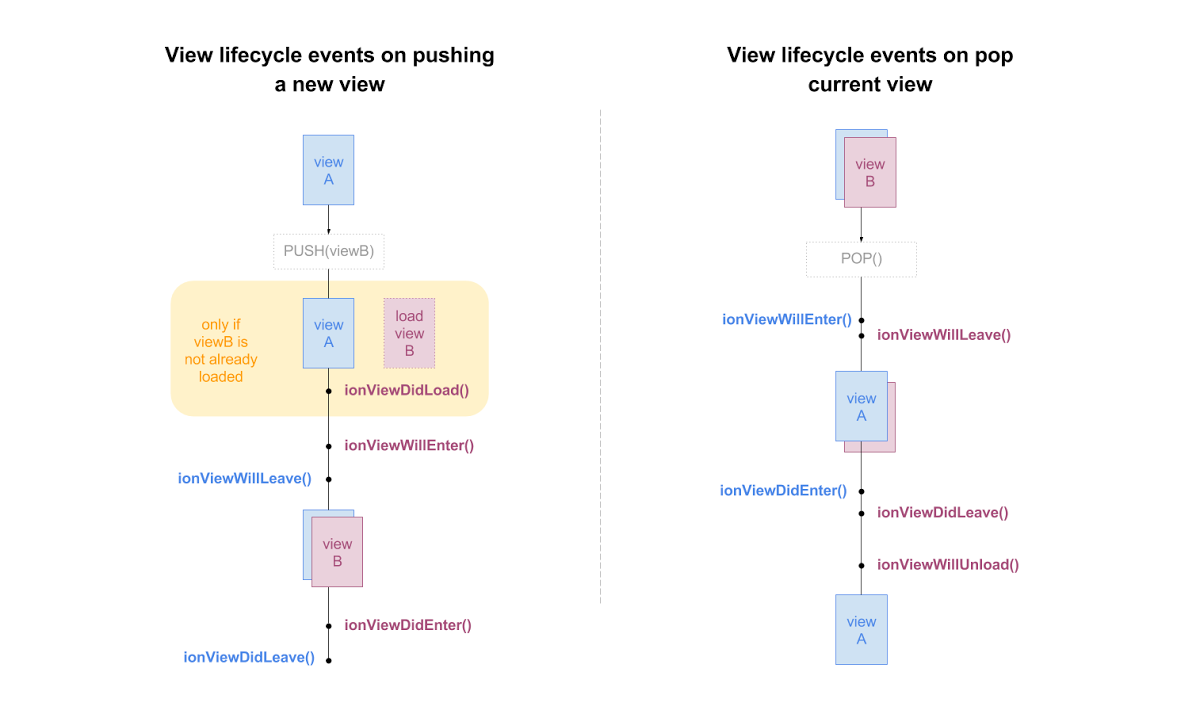
\includegraphics[width=\textwidth]{ionicViewLifecycleEvents}
    }%
    }%
    \caption{Ionic view Lifecycle Events \cite{Ionic_lifecycle}.}
    \label{fig:IonicViewLifecycleEvents}
\end{figure}
\noindent
Por último, para ir probando la aplicación tenemos dos opciones. Por un lado usando la primera orden de \textit{Ionic} que se muestra a continuación, que nos permite de manera rápida mostrar la interfaz de la aplicación en las distintas plataformas.
O bien realizar un despliegue en la plataforma en concreto, lo cual nos permite compilar la aplicación como proyecto correspondiente a la plataforma donde la estamos desplegando.
En nuestro caso cuando la lancemos en Android se generará una carpeta dentro de \texttt{platforms/} que contendrá un proyecto de Android Studio, o en el caso de iOS un proyecto de XCode. 

\begin{lstlisting}
    Ionic serve --lab
    Ionic cordova run android
\end{lstlisting}
